\documentclass{standalone}
\usepackage{tikz}
\begin{document}
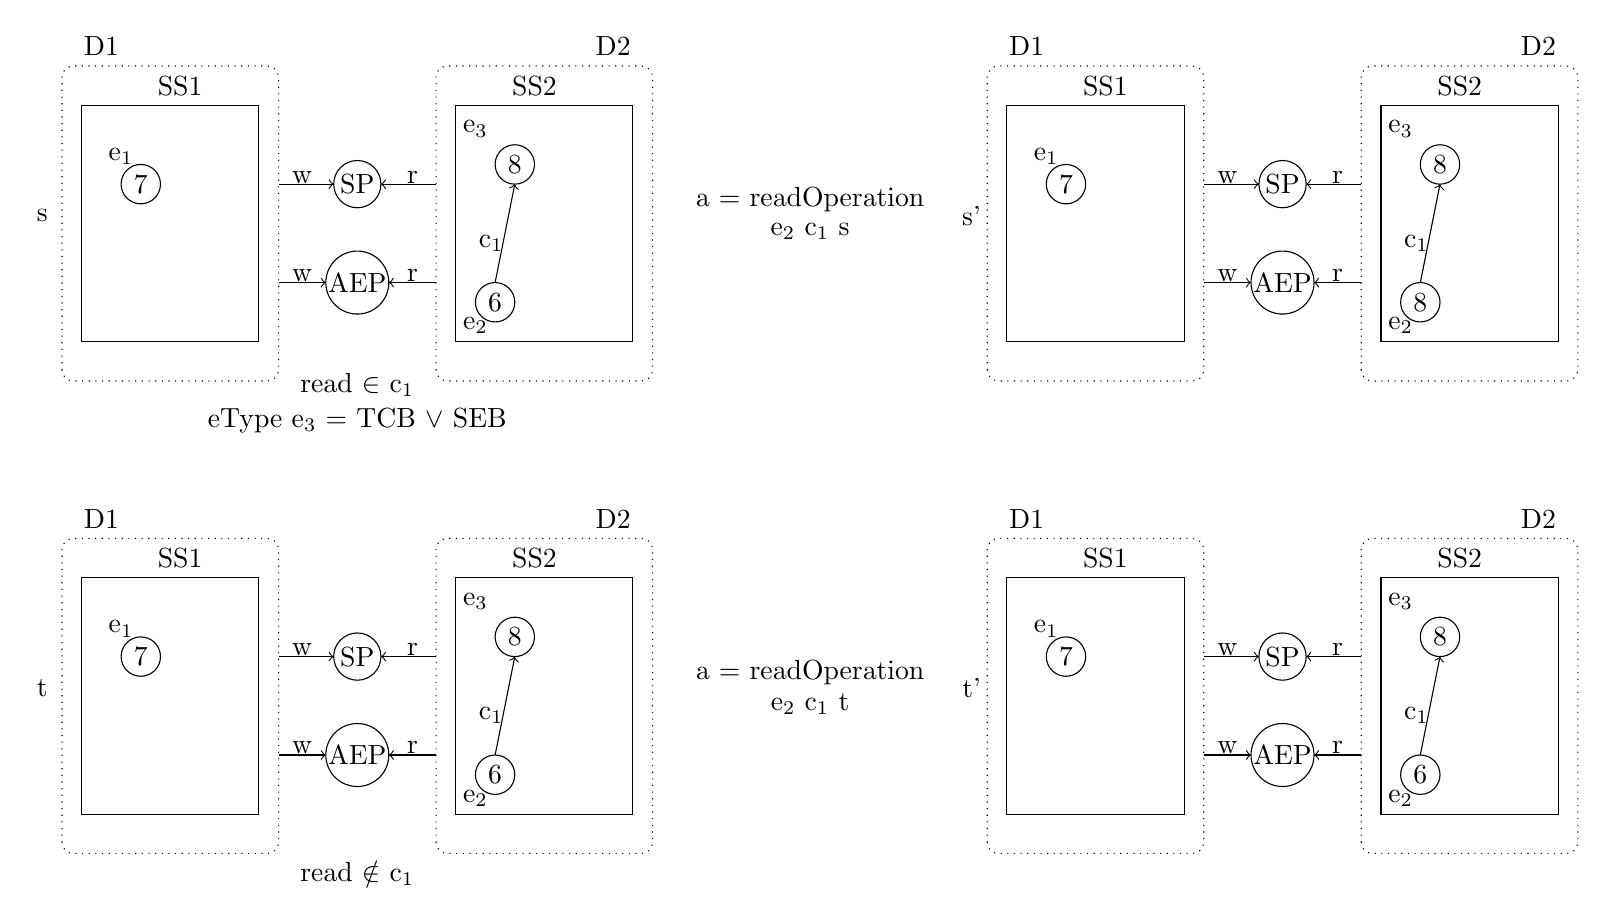
\begin{tikzpicture}
\node at (-0.25,1.6) {t};
\node at (1.5,3.25) {SS1};
\node at (0.5,3.75) {D1};
\node at (7,3.75) {D2};
\draw [black, dotted, rounded corners] (0,-0.5) rectangle (2.75,3.5);
\draw [black] (0.25,0) rectangle (2.5,3);
\draw [black, dotted, rounded corners] (4.75,-0.5) rectangle (7.5,3.5);
\draw [black] (5,0) rectangle (7.25,3);
\draw [black] (1,2) circle [radius=0.25] node {7};
\node at (0.75,2.35) {e$_1$};
\node at (6,3.25) {SS2};
\node at (5.25,2.7) {e$_3$};
\draw [black] (5.75,2.25) circle [radius=0.25] node {8};
\draw [black] (5.5,0.5) circle [radius=0.25] node {6};
\node at (5.25,0.2) {e$_2$};
\draw [->, black] (5.5,0.75) -- (5.75,2);
\node at (5.45,1.25) {c$_1$};
\node at (3.75,-0.75) {read $\notin$ c$_1$};
\node at (9.5,1.8) {a = readOperation};
\node at (9.5,1.4) { e$_2$ c$_1$ t};
\draw [black] (3.75,0.75) circle [radius=0.4] node {AEP};
\draw [black] (3.75,2) circle [radius=0.3] node {SP};
\draw [->, black] (2.75,0.75) -- (3.35,0.75);
\draw [<-, black] (4.15,0.75) -- (4.75,0.75);
\node at (3.05,0.84) {w};
\node at (4.45,0.84) {r};
\draw [->, black] (2.75,2) -- (3.45,2);
\draw [<-, black] (4.05,2) -- (4.75,2);
\node at (3.05,2.09) {w};
\node at (4.45,2.09) {r};

\node at (11.55,1.6) {t'};
\node at (12.25,3.75) {D1};
\node at (18.75,3.75) {D2};
\node at (13.25,3.25) {SS1};
\draw [black, dotted, rounded corners] (11.75,-0.5) rectangle (14.5,3.5);
\draw [black] (12,0) rectangle (14.25,3);
\draw [black, dotted, rounded corners] (16.5,-0.5) rectangle (19.25,3.5);
\draw [black] (16.75,0) rectangle (19,3);
\draw [black] (12.75,2) circle [radius=0.25] node {7};
\node at (12.5,2.35) {e$_1$};
\node at (17.75,3.25) {SS2};
\node at (17,2.7) {e$_3$};
\draw [black] (17.5,2.25) circle [radius=0.25] node {8};
\draw [black] (17.25,0.5) circle [radius=0.25] node {6};
\node at (17,0.2) {e$_2$};
\draw [->, black] (17.25,0.75) -- (17.5,2);
\node at (17.2,1.25) {c$_1$};
\draw [black] (15.5,0.75) circle [radius=0.4] node {AEP};
\draw [black] (15.5,2) circle [radius=0.3] node {SP};
\draw [->, black] (14.5,0.75) -- (15.1,0.75);
\draw [<-, black] (15.9,0.75) -- (16.5,0.75);
\node at (14.8,0.84) {w};
\node at (16.2,0.84) {r};
\draw [->, black] (14.5,2) -- (15.2,2);
\draw [<-, black] (15.8,2) -- (16.5,2);
\node at (14.8,2.09) {w};
\node at (16.2,2.09) {r};

\node at (-0.25,7.6) {s};
\node at (1.5,9.25) {SS1};
\node at (0.5,9.75) {D1};
\node at (7,9.75) {D2};
\draw [black, dotted, rounded corners] (0,5.5) rectangle (2.75,9.5);
\draw [black] (0.25,6) rectangle (2.5,9);
\draw [black, dotted, rounded corners] (4.75,5.5) rectangle (7.5,9.5);
\draw [black] (5,6) rectangle (7.25,9);
\draw [black] (1,8) circle [radius=0.25] node {7};
\node at (0.75,8.35) {e$_1$};
\node at (6,9.25) {SS2};
\node at (5.25,8.7) {e$_3$};
\draw [black] (5.75,8.25) circle [radius=0.25] node {8};
\draw [black] (5.5,6.5) circle [radius=0.25] node {6};
\node at (5.25,6.2) {e$_2$};
\draw [->, black] (5.5,6.75) -- (5.75,8);
\node at (5.45,7.25) {c$_1$};
\node at (3.75,5.45) {read $\in$ c$_1$};
\node at (3.75,5) {eType e$_3$ = TCB $\vee$ SEB};
\node at (9.5,7.8) {a = readOperation}; 
\node at (9.5,7.4) {e$_2$ c$_1$ s};
\draw [black] (3.75,6.75) circle [radius=0.4] node {AEP};
\draw [black] (3.75,8) circle [radius=0.3] node {SP};
\draw [->, black] (2.75,6.75) -- (3.35,6.75);
\draw [<-, black] (4.15,6.75) -- (4.75,6.75);
\node at (3.05,6.84) {w};
\node at (4.45,6.84) {r};
\draw [->, black] (2.75,8) -- (3.45,8);
\draw [<-, black] (4.05,8) -- (4.75,8);
\node at (3.05,8.09) {w};
\node at (4.45,8.09) {r};

\node at (11.55,7.6) {s'};
\node at (12.25,9.75) {D1};
\node at (18.75,9.75) {D2};
\node at (13.25,9.25) {SS1};
\draw [black, dotted, rounded corners] (11.75,5.5) rectangle (14.5,9.5);
\draw [black] (12,6) rectangle (14.25,9);
\draw [black, dotted, rounded corners] (16.5,5.5) rectangle (19.25,9.5);
\draw [black] (16.75,6) rectangle (19,9);
\draw [black] (12.75,8) circle [radius=0.25] node {7};
\node at (12.5,8.35) {e$_1$};
\node at (17.75,9.25) {SS2};
\node at (17,8.7) {e$_3$};
\draw [black] (17.5,8.25) circle [radius=0.25] node {8};
\draw [black] (17.25,6.5) circle [radius=0.25] node {8};
\node at (17,6.2) {e$_2$};
\draw [->, black] (17.25,6.75) -- (17.5,8);
\node at (17.2,7.25) {c$_1$};
\draw [black] (15.5,6.75) circle [radius=0.4] node {AEP};
\draw [black] (15.5,8) circle [radius=0.3] node {SP};
\draw [->, black] (14.5,6.75) -- (15.1,6.75);
\draw [<-, black] (15.9,6.75) -- (16.5,6.75);
\node at (14.8,6.84) {w};
\node at (16.2,6.84) {r};
\draw [->, black] (14.5,8) -- (15.2,8);
\draw [<-, black] (15.8,8) -- (16.5,8);
\node at (14.8,8.09) {w};
\node at (16.2,8.09) {r};
\end{tikzpicture}
\end{document}
